\nsection{Draw to Unlock}

Rather than remembering passwords or passcodes, many mobile
devices now allow the user to draw a pattern on the screen to
unlock them.
\begin{center}
\scalebox{0.5}{
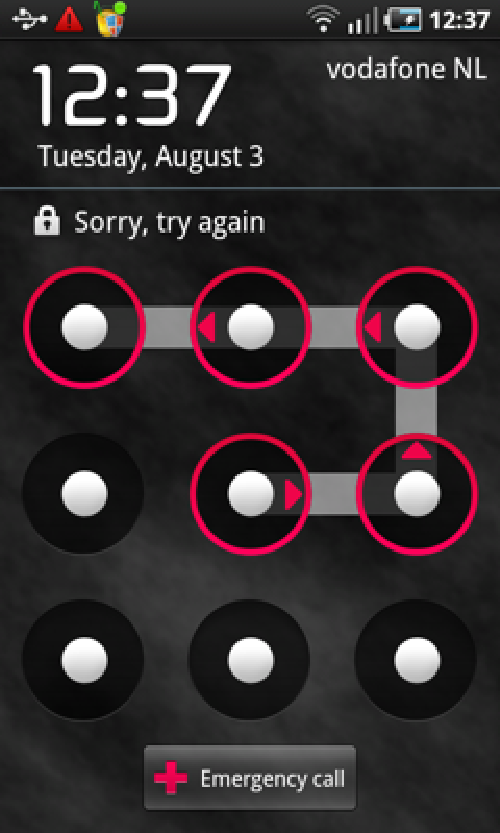
\includegraphics{./phonelock.pdf}
}
\end{center}

Here we will explore how many unique patterns are available
when drawing such patterns to connect ``dots'', such as shown in the
figure.
We assume that people put their finger on one ``dot'' and then only ever move
one position left, right, up or down (but never diagonally) at
a time. You are not allowed to return to a ``dot'' once it has
been visited once. If we number the first position in our path as $1$, the
second as $2$ and so on, then beginning in the top left-hand
corner, some of the possible patterns of 9 moves are~:
\begin{verbatim}

1 2 3      1 2 3      1 2 3
6 5 4      8 9 4      8 7 4
7 8 9      7 6 5      9 6 5

\end{verbatim}

\begin{exercise}
Write a program that computes and outputs all the valid paths.
Use \textbf{recursion} to achieve this.
\begin{itemize}
\item How many different patterns of length $9$ are
    available on a $3 \times 3$ grid, if the user begins in
    the top left corner~?

\item How many different patterns of length $9$ are
    available on a $3 \times 3$ grid, if the user begins in
    the middle left~?

\item How many different patterns of length $7$ are
    available on a $3 \times 3$ grid, if the user begins in
    the top left corner~?

\item How many different patterns of length $25$ are
    available on a $5 \times 5$ grid, if the user begins in
    the top left corner~?
\end{itemize}
\end{exercise}
